%!TEX ROOT = thesis.tex
\chapter{THEORETICAL FRAMEWORK}
\label{chap: 3}

In this chapter we would start with a brief history of artificial intelligence research that are directly or indirectly related to the innovation of transformers. Then, the second section would covers the foundations of deep learning which includes feed-forward neural networks, activation functions, loss functions and evaluation metric. The third section would cover the basics of transformers. The final section would include the potential challenged of this project.

\section{A Brief History of Deep Learning}

Modern deep learning as we know it today can be traced back to when Frank Rosenblatt introduced the perceptron in 1959, referring to it as the "Mark I Perceptron" shown in figure \ref{fig:perceptron}. Given an input, the perceptron will generate an output based on a linear thresholding logic. The weights in the perceptron were updated and learned by iteratively reducing the difference between the generated output and the desired output and passing in a new input.

The perceptron never took off in popularity because Marvin Minsky and Seymour Papert showed the limitations of perceptrons in learning the simple XOR function. In 1986, David Rumelhart, Geoff Hinton, and Ronald Williams showed how by incorporating "hidden" layers, a multi-layer perceptron can be used to overcome the weakness of perceptrons in learning complex patterns. Multi-layer perceptrons are also known as neural networks.

\begin{figure}[ht]
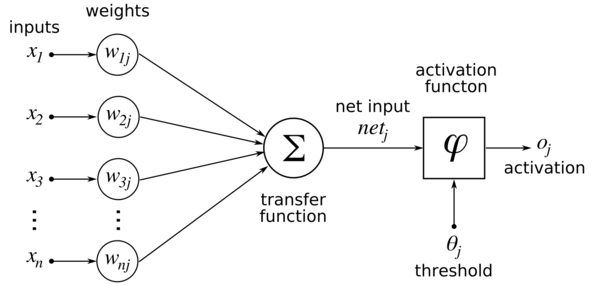
\includegraphics[width=10.5cm, height=5.5cm]{images/Rosenblattperceptron.png}
\centering
\caption{Rosenblatt Perceptron}
\label{fig:perceptron}
\end{figure}

LeCun et al., published a method to recognized hand-written digits and it was utilized bythe U.S. Postal Service \cite{LeCunBoserDenkerEtAl89}, making it the first neural network model that received widesread adoption . This is a huge milestone for deep learning, proving the usefulness of convolution operations and weight learning the features in computer vision.

However, there are still a lot of flaws with neural networks. Take for example backpropagation, the weight learning algorithm in neural networks, has a number of issues such as vanishing gradients, exploding gradients, and the inability to learn long-term information. Hochreiter and Schmidhuber showed how  Long short-term memory (LSTM) architecture could overcome shortcomings of backpropagation over time.

LeCun et al. also showed the advantages of deep learning through more complex neural networks architectures such as convolutional neural networks (CNNs), restricted Boltzmann machines (RBMs), and deep belief networks (DBNs). They also showed the importance of techniques such as unsupervised pre-training
with fine-tuning, thus inspiring the next wave of deep learning. Li et al.,  launched ImageNet, which was the most extensive collection of labelled images and highlighted the importance of robust dataset to train a deep learning model for computer vision task. 

Mikolov et al. and Graves proposed language models using Recurrent Neural Networks (RNN) and LSTM, which later became the building blocks for many natural language processing (NLP) architectures. Sequence-to-sequence framework became the core architecture for a wide range of NLP tasks. Bahdanau et al. proposed the attention mechanism to overcome the bottleneck issue with sequence-tosequence model. Attention mechanismplays a crucial role in subsequent evolution of Transformers.

In 2017, Transformers were formally introduced in the "Attention is All You Need" paper \cite{attention-is-all-you-need} and became the most popular architecture in NLP. In 2020, Vision Transformers \cite{16x16} introduced a method to adapt Transformers for computer vision by splitting the input image into patches and represent them as vectors.


\section{Theoretical Introduction to Deep Learning}
\subsection{Convolutional Neural Networks and Its Application in Semantic Segmentation of Satellite Images}

U-net, semua CNN jadah masuk sini.
\subsubsection{Activation Functions}
Sigmoid, RELU, softmax

\section{Introduction to Transformers}\label{subsection:Intro to Trans}
\subsection{Encoder-Decoder Architecture}
\subsection{Sequence-To-Sequence}
\subsection{Attention Mechanism}
\subsection{Embedding and Positional Encoding}
\subsection{sdsds}\label{sasas}
\section{Transformers Architecture}
%%%%%%%%%%%%%%%%%%%%%%%%%%%%%  ViT
\subsection{Vision Transformer (ViT)}
Vision Transformer from \cite{16x16} is the first group of researchers that experimented with Vision Transformer by applying a standard Transformer directly to images, with the fewest possible modifications. Their model is known as Vision Transformer (ViT) as it is the first Vision Transformer. They split an image into patches and provide the sequence of linear embeddings of these patches as an input to a Transformer. The image patches were treated the same way as word tokens do in an NLP application. This methods fails to capture the  translation equivariance and locality provide by the CNNs hence it is unsuitable for semantic segmentation task.

Another issue with Vision Transformer is the attention mechanism itself is $O(n^2)$ because it is a dot product thus requiring it to consume significant computational time and memory to capture the global context, which in turn, reducing its efficiency, scaling potential and its potential for real-world applications. Figure \ref{fig:vit} shows the ViT architecture.

\begin{figure}[ht]
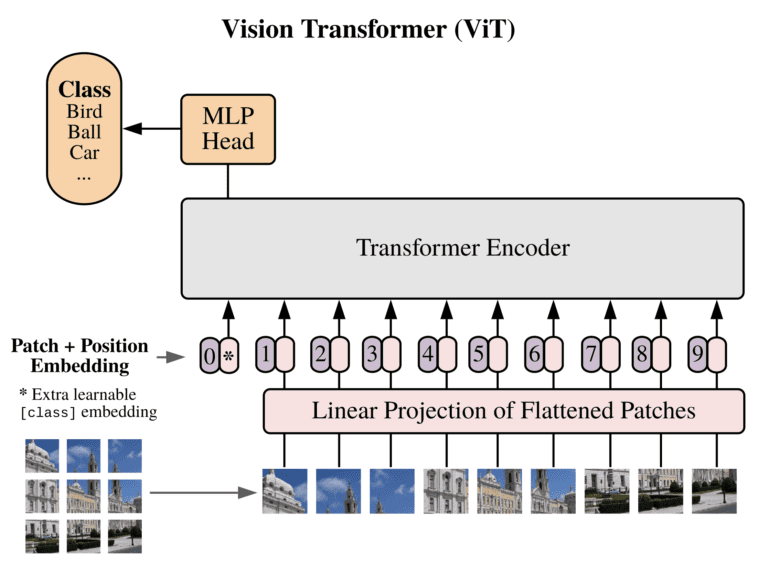
\includegraphics[width=13.5cm, height=9cm]{images/vision transformer.png}
\centering
\caption{ViT Architecture}
\label{fig:vit}
\end{figure}

%%%%%%%%%%%%%%%%%%%%%%%%%%%%%  Swin V1 and V2
\subsection{Swin Transformer}
The first version of Swin Transformer \cite{swin-v1} presents a hierarchical feature representation scheme that demonstrates impressive performances with linear computational complexity, which makes it suitable for semantic segmentation. The detailed mechanism of Transformers and Vision Transformers are discussed in chapter \ref{chap: 3}.

\FloatBarrier
\begin{figure}[ht]
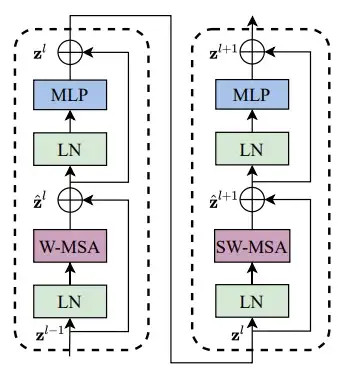
\includegraphics[width=9.5cm, height=7cm]{images/swin-architecture.jpg}
\centering
\caption{Swin Transformer V1 Architecture}
\label{fig:swin architecture}
\end{figure}

\begin{figure}[ht]
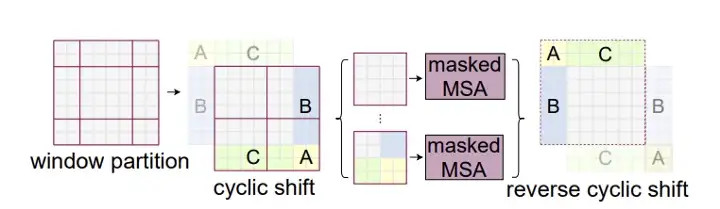
\includegraphics[width=13.5cm, height=5.5cm]{images/swin-cyclic-shift.jpg}
\centering
\caption{Cyclic Shifted Windows in Swin Transformer}
\label{fig:swin cyclic}
\end{figure}

\FloatBarrier
\begin{figure}[ht]
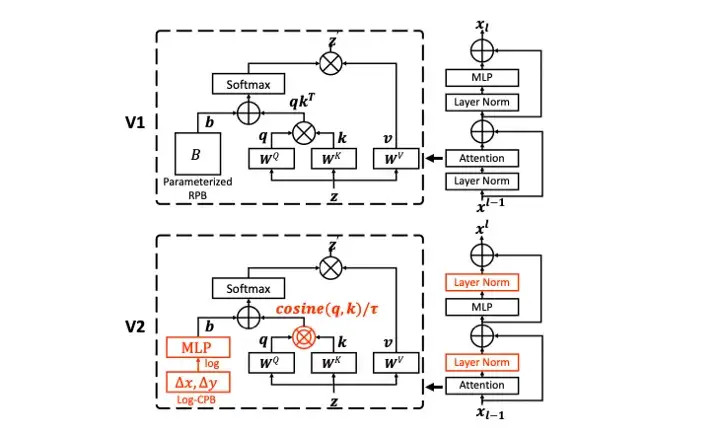
\includegraphics[width=13.5cm, height=9.5cm]{images/swin1-vs-swin2.jpg}
\centering
\caption{Difference Between Swin V1 and Swin V2}
\label{fig:swin v1 vs v2}
\end{figure}
\FloatBarrier

%%%%%%%%%%%%%%%%%%%%%%%%%%%%%  SegFormer
\subsection{SegFormer}

%%%%%%%%%%%%%%%%%%%%%%%%%%%%%  MaskFormer
\subsection{MaskFormer}

%%%%%%%%%%%%%%%%%%%%%%%%%%%% Beit
\subsection{Beit}

%%%%%%%%%%%%%%%%%%%%%%%%%%%%% DeeepLabV3
\subsection{DeepLabV3}
\section{Evaluation Metrics}
\section{Limitations}

\subsection{Weak Supervision}
\cite{weakly-supervised-semantic} identified that a lot of semantic segmentation models doesn't work well under weak supervision. In this paper weak supervision is defined as using dataset that fulfil at least one of this criteria:
\begin{enumerate}
    \item \textit{Incomplete supervision} - The dataset is small and insufficient to train a good model.
    \item \textit{Inexact supervision} - The labelling is not as exact as necessary which usually occurss in land cover labels with low resolution.
    \item \textit{Inaccurate supervision} - The labels are wrong.
\end{enumerate}

\subsection{Inadequate Computing Resource}

